\chapter{基礎知識と課題整理}
\label{chap:background}

\section{sXGPと4G/5Gの概要}
\subsection{sXGPの位置づけ(免許不要・TD-LTE互換)}
本節では、sXGPの制度的位置づけ(免許不要帯・チャネル幅・出力制限など)とTD-LTE互換性、利用可能な端末・eNB機器、研究/教育用途における利点と限界を概説する。
\subsection{4G RAN(UE・eNB)とEPC/5GCの要素}
UE/eNB/EPCの基本構成と主要インタフェース(Uu, S1-MME, S1-U)、RRCとNASの役割、Attach/認証/セッション確立の要点を整理する。
\subsection{5GCのアーキテクチャ(AMF/SMF/UPF等)}
AMF/SMF/UPF/UDM/AUSF/NRFなどの機能分担とNインタフェース、登録・セッション管理・ポリシ適用の流れを俯瞰し、本研究で利用する機能範囲を明確化する。

\section{3GPP標準化と標準-実装ギャップ}
\subsection{仕様の包含範囲とリファレンス実装の不足}
3GPP仕様の階層(SA/CT/RAN)と各TSの対象範囲、必須/任意要件や相互参照の構造、実装上の曖昧点(未規定項目)の例を挙げ、研究への影響を指摘する。
\subsection{ベンダ実装差と相互接続性の課題}
ベンダ実装差の典型(IEの扱い、タイマ既定値、再送・フォールバック、ベンダ拡張IE)とIOTで顕在化する問題、既知の回避策/ベストプラクティスを述べる。
\subsection{研究・評価におけるギャップの影響}
仕様―実装ギャップが再現性・比較可能性に与える影響、論文実験の内的/外的妥当性への波及、OSSでギャップを埋める方針を示す。

\section{RAN–コア間インターワーキングの基礎}
\subsection{制御面(S1-AP vs. NG-AP)}
S1-APとNG-APのメッセージ対応関係、登録/セッション確立に関わる必須IE、エラー/例外時の取り扱い、コンバータにおける変換ポイントを列挙する。
\subsection{ユーザ面(GTP-U互換性とパススルー/変換)}
GTP-Uのトンネル管理(TEID割当・再利用)、MTU/フラグメント、順序/再送の扱い、QoS/5QI対応、UPF経由時のパスを整理する。
\subsection{ID/コンテキスト管理(NAS, IMSI/SUPI 等)}
IMSI/SUPI, GUTI/5G-GUTIなどの識別子、NASセキュリティコンテキスト(KDF, KAMF/KNASint/KNASenc)の概要と、コンバータ内でのマッピング/生存期間管理方針を述べる。

\section{OSSと6Gに向けた開発・検証サイクル}
\subsection{OSSの役割(Open5GS等)と試作の加速}
Open5GS等OSSコアの構成と拡張性、コミュニティ/CIの活用、研究プロトタイプの実装速度や学習コスト低減の利点をまとめる。
\subsection{適合・相互接続・回帰テストの自動化}
自動試験の枠組み(シナリオ駆動、pcap/ログ照合、差分検出)と既存テスト資産の参考例(TTCN-3等)、回帰の最小セット設計を記す。
\subsection{再現性(Docker等)と研究公開の促進}
コンテナ化・固定バージョン・seed/設定共有、データ/成果物の保存と再実行手順、公開時の留意点(鍵や個人情報の除去)を簡潔に示す。

\section{モバイルシステム全体での課題感}
\subsection{研究環境のコストとライセンス(免許・機器費用)}
端末/モデム/eNB/SDR/アンテナ/測定機器の費用感、免許や試験局の手続き、sXGP採用によるコスト/手続き削減効果を見積もる。
\subsection{相互接続性・ベンダ依存の壁}
UE/モデム/OS/カーネル/NIC差やRAN/コアのベンダ差が及ぼす影響例を列挙し、評価設計での緩和策(多端末/多実装での検証)を書く。
\subsection{運用・再現性とオープンテストベッドの不足}
共有可能なテストベッドの不足と再現性の課題、提供したいアーティファクト(構成・スクリプト・パケットトレース)を述べる。
\subsection{セキュリティ・計測基盤の一般化の難しさ}
鍵/認証情報の取り扱い、プライバシ/PII、攻撃面の考慮、計測オーバーヘッドと観測者効果の抑制を整理する。

\section{法規制とsXGPの位置づけ}
\subsection{電波法の制約と実機検証の困難}
屋内外・出力・使用帯域・電波暗室等の制約、干渉リスク、学術機関での典型的な許認可フローを概説する。
\subsection{免許不要帯を用いた代替アプローチとしてのsXGPの意義}
sXGPにより合法かつ安全に実機相当のRAN検証を行う意義と限界(周波数・設備可用性・スループット等)を要約する。

\section{シミュレータの対象範囲と限界}
\subsection{シミュレーションで十分な領域}
新NFのアルゴリズム検討、プロトコル状態機械の基本遷移の正当性確認、ラフなスケール試験、CIでの高速回帰などはシミュレータで効率的に実施できる。
\subsection{シミュレーションの限界}
実UE固有の実装差(RRC/NASのタイマ・再送・Capability差)、RRC/PHY/MACの時間ゆらぎ由来の境界条件、OS/NICのオフロードやキューイング、パケット順序入替・フラグメンテーション、S1AP$\leftrightarrow$NGAP変換やTEID管理の例外パスなどは、シミュレータでは再現が難しい。

\section{実機が必要となる検証項目}
\begin{itemize}
	\item 厳密なタイマ境界・再送・例外遷移(登録/PDU確立、NAS/RRCの異常系)
	\item セキュリティと鍵管理(AKA/EAP-AKA'、KDF、再同期、アルゴ協定の実装差)
	\item ユーザ面の実性能(GTP-Uオフロード、カーネル/DPDK、NUMA/CPUスケジューリング)
	\item 相互接続・回帰(複数UE/モデム/OSでの互換性検証)
	\item フェイルシナリオ(部分ロス、遅延、再順序化、NICドロップ、CPUスタベーション)
\end{itemize}

\section{本環境がもたらす価値(ユースケース)}
\label{sec:values}
\subsection{教育・トレーニング}
免許不要帯で運用可能なsXGPをeNBとして活用し、4G RANと5GCを接続できるため、学部・大学院・企業研修において、法令遵守のもとで実機に近い無線・コア連携の学習が可能となる。設定の再現手順を公開することで、実験レポートの客観性と再現性も高められる。

\subsection{プロトタイピングと検証の高速化}
コントロールプレーン(S1AP/NGAP/NAS)およびユーザプレーン(GTP-U)の変換・中継部を差し替え可能にすることで、新しいアルゴリズムやポリシー(例:識別子管理、TEID割当、タイムアウト制御)の試作・検証を低コストで繰り返し実施できる。

\subsection{相互接続・回帰テスト}
Open5GSなどの5GC実装や各種eNB/UEに対して、信令互換性や基本機能(登録、PDUセッション確立)の回帰テストを自動化できる。コンバータを介した差分吸収により、ベンダ差や仕様差を可視化しつつ評価できる。

\subsection{性能評価とボトルネック分析}
遅延・スループット・リソース使用率(CPU/メモリ)の計測基盤を同梱することで、コンバータの処理遅延やカプセル化オーバヘッド、TEID管理戦略の影響を定量化でき、設計改善に資する。

\subsection{再現性の高い研究公開と共同研究}
Dockerを用いた構成管理とビルド手順の統一により、第三者が同一環境で追試できる。研究成果の普及や共同研究の立ち上げコストを下げる。

\subsection{運用研究・障害シナリオの再現}
認証失敗やセキュリティモードエラー、ハンドオーバ相当の遷移など、現場で発生しうる事象の再現とトラブルシュート手順の確立に役立つ。

\section{本研究が対象とする課題の定義}
\subsection{研究者・学生が手軽に再現できる環境の要件}
必要構成要素・費用・所要時間・依存関係・再現手順の粒度を定義し、到達すべきユーザ体験(セットアップから成功確認まで)を示す。
\subsection{sXGP×5GC接続の技術的論点の範囲}
本研究で扱う範囲(制御/ユーザ面の変換、識別子/セキュリティ/状態管理)と扱わない範囲(RRC/PHY最適化、商用品質の最適化など)を明確化する。
\subsection{評価指標と成功基準の設定}
機能(登録/セッション確立率)、性能(遅延/スループット/CPU等)、堅牢性(異常時の復帰)、再現性(環境差耐性)の指標と合格基準を定める。


% (注)宇宙通信に関する章は本研究スコープ外のため削除。

% (注)該当節を削除。


% (注)該当節を削除。


% (注)該当節を削除。

% (注)DTN記述は別研究のため削除。

% \subsection{通信機会の非対称性}
% \label{subsection:通信機会の非対称性}

% \begin{figure}[tbh]
%     \centering
%     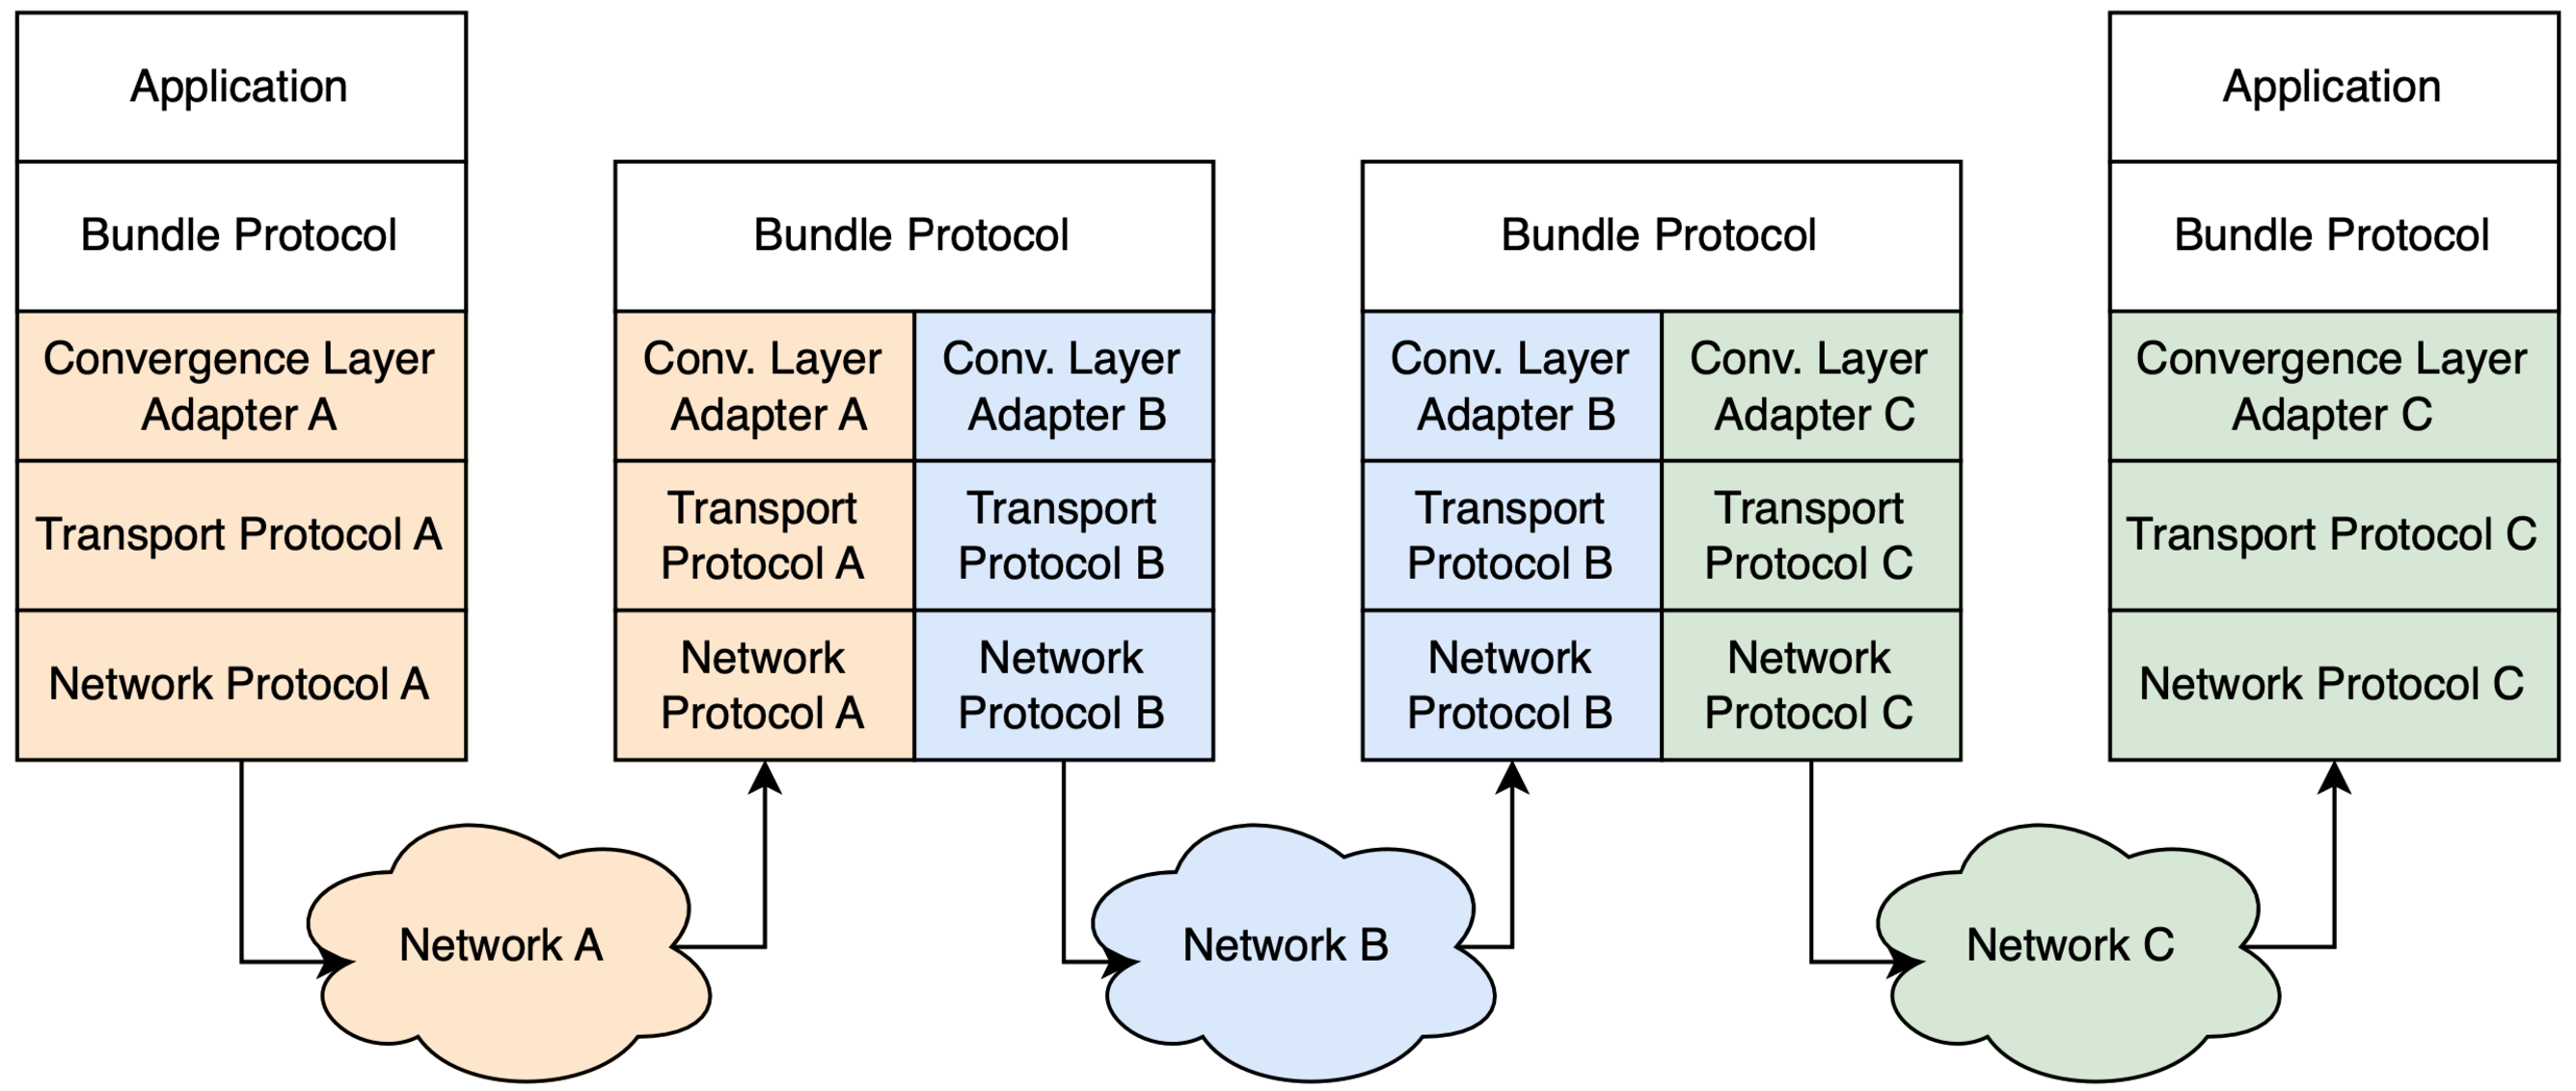
\includegraphics[width=0.7\textheight]{img/dtnprotocolstack.pdf}
%     \caption{DTNを搭載したノード間のみでの通信}
%     \label{fig:dtnprotocolstack}
%     \begin{minipage}{\textwidth}
%         \raggedright
%         \vspace{3mm}
%         \fontsize{10.5pt}{12pt}\selectfont
%         参考文献\cite{bundle_protocol_architecture}Figure1をもとに作成.
%         図中のConvergence Layer(CL)については
%         \ref{section:Convergence LayerとLTP}項で説明する.
%     \end{minipage}
% \end{figure}

% (注)該当節を削除。

% (注)該当節を削除。

% (注)該当節を削除。

% (注)該当節を削除。

% (注)該当節を削除。

% \begin{table}[tbh]
%     \centering
%     \caption{DTN実装とその機能の比較}
%     \begin{minipage}[t]{\textwidth}
%         \centering
%         \fontsize{10.5pt}{12pt}\selectfont
%         参考文献\cite{dtn_implementations}figure1より抜粋
%         \vspace{3mm}
%     \end{minipage}
%     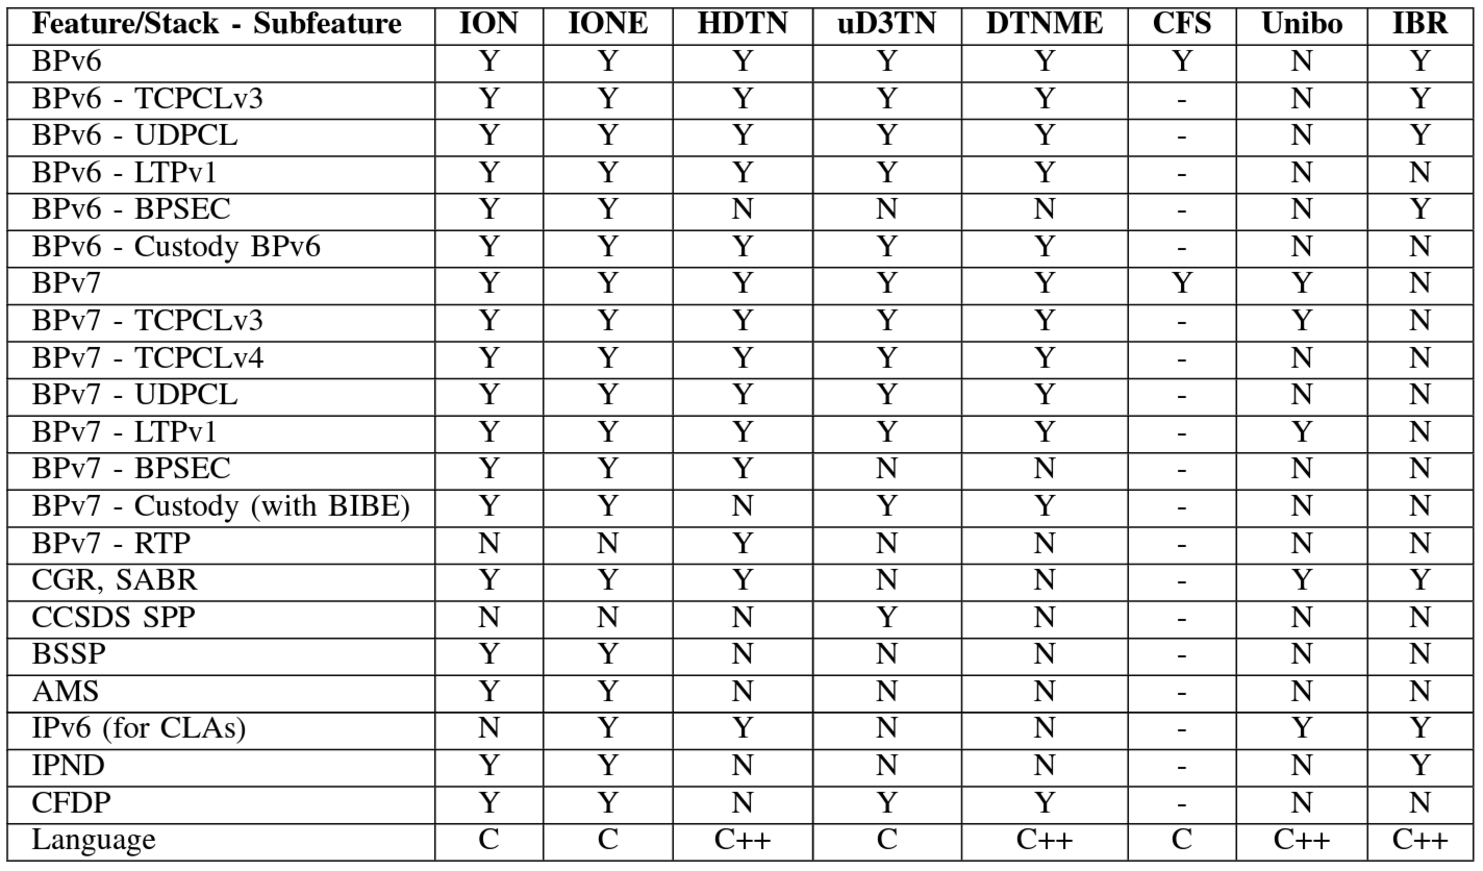
\includegraphics[width=0.7\textheight]{img/chart_dtn_implementations.pdf}
%     \label{table:chart_dtn_implementations}
% \end{table}
